\documentclass[11pt]{article}
\usepackage[letterpaper,margin=1in]{geometry}
\usepackage{color}
\usepackage[dvipdfmx]{graphicx}
\usepackage{amsbsy}
\usepackage{amssymb}
\usepackage{amsmath}
\usepackage{adjustbox}
\usepackage{url}
\usepackage{mathtools}
\DeclarePairedDelimiter\ceil{\lceil}{\rceil}
\DeclarePairedDelimiter\floor{\lfloor}{\rfloor}

\newcommand{\argmax}{\mathop{\rm arg~max}\limits}
\newenvironment{claim}[1]{\par\noindent\underline{Claim:}\space#1}{}
\newenvironment{claimproof}[1]{\par\noindent\underline{Proof:}\space#1}{\hfill $\blacksquare$}


\begin{document}
\title{Analysis Report on Assignment 5: PAC Learnability}
\author{Yoshinari Fujinuma}
\date{}
\maketitle

\section{Problem 1}
% http://grandmaster.colorado.edu/~cketelsen/files/csci5622/videos/lesson12/lesson12.pdf
The problem 1 is to determine the minimum number of training examples $m$ for ``any consistent learner using $H=C$ will, with probability $95\%$, output a hypothesis with error at most $0.15$''. In other  words we want know the minimum number of training examples necessary to accomplish with the error $\epsilon = 0.15$, and the confidence $\delta = 0.05$

The number of hypothesis $|H|$ is any combinations of three different points, where $N$ is the number of possible points $(x, y)$ in $x \in [0, 99]$ and $y \in [0, 99]$. So $N = 100 * 100 = 10,000$, and the number of hypothesis is
$$
|H| = \dbinom{N}{3} = 166,616,670,000.
$$

According to Lecture 12\footnote{http://grandmaster.colorado.edu/~cketelsen/files/csci5622/videos/lesson12/lesson12.pdf}, the concept $c$ is PAC learnable with 
$$
m \geq \frac{1}{\epsilon}(\ln |H| + \ln(\frac{1}{\delta}))
$$
By plugging in $\epsilon = 0.15$ and $\delta = 0.05$, 
$$
m \geq \frac{1}{0.15}(\ln(166,616,670,000) + \ln(\frac{1}{0.05})) \approx 192.23
$$
So the bound or the minimum number of training examples necessary is $m = \ceil{192.23} = 193$.


\section{Problem 2}
Problem statement: ``State and prove the VC Dimension of the hypothesis class H of linear hyperplanes in 2D that pass through the origin.''

According to Lecture 13\footnote{http://grandmaster.colorado.edu/~cketelsen/files/csci5622/videos/lesson13/lesson13.pdf}, the VC dimension is defined as the following:
$$
\mbox{VCdim}(H) = max\{|S|: H \mbox{ shatters } S \mbox{ for some } S\}
$$

The distance $d$ of a point $(x_i, y_i)$ from a line $y = ax$ is
$$
d = \frac{|ax_i - y_i|}{\sqrt{a^2 + 1}}.
$$

The decision boundary given a line $y = ax$ is
$$ 
h(x_i, y_i) = \begin{cases} 
%          +1 \mbox{ if } 0 \geq ax - y \geq 1 \mbox{ (i.e. above the line) }\\
%          -1 \mbox{ else } ax - y < 0 \mbox{ (i.e. below the line) }\\
          +1 \mbox{ if } 0 \leq d = \frac{|ax_i - y_i|}{\sqrt{a^2 + 1}} \leq 1 \mbox{ (i.e. The distance of a point $(x_i, y_i)$ from the line $y = ax$ is $\leq 1$) }\\
          -1 \mbox{ else }\\
\end{cases}
$$

\subsection{Proof of the lower bound}
\label{lowerbound}

For a given $2$ points in 2D, we can shatter in similar way to slides 22 through 25. See Figures 1, 2, 3, and 4.

\begin{figure}[htb]
  \begin{center}
   \begin{tabular}{c}
    \begin{minipage}{0.5\hsize}
     \begin{center}
     \scalebox{0.33}
      {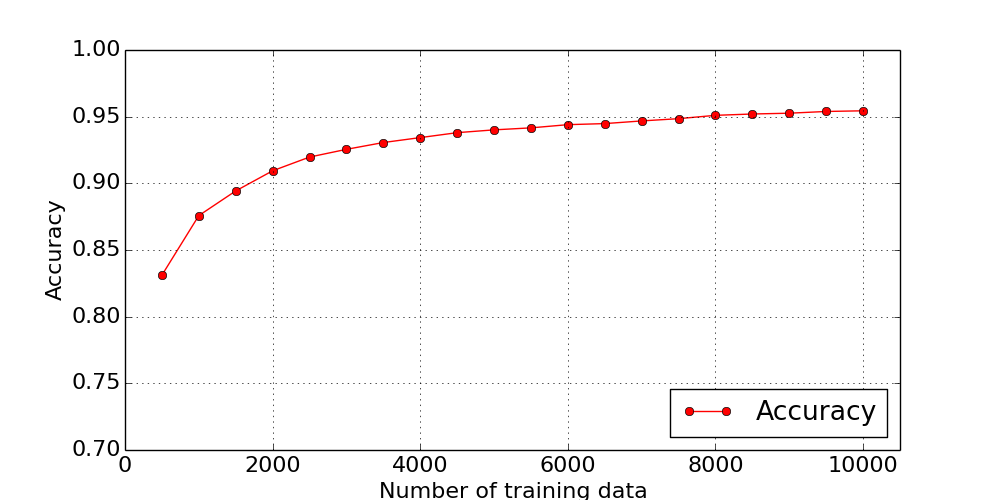
\includegraphics[]{figure_1.png}}
   
      \caption{$a = 4/5$. }
      \label{fig:1}
     \end{center}
    \end{minipage}

    \begin{minipage}{0.01\hsize}
    \end{minipage}

    \begin{minipage}{0.5\hsize}
     \begin{center}
      \scalebox{0.33}
      {\includegraphics[]{figure_3.png}}
      \caption{\label{fig:2} $a = 5/2$}
     \end{center}
    \end{minipage}

  \end{tabular}
 \end{center}
\end{figure}

\begin{figure}[htb]
  \begin{center}
   \begin{tabular}{c}
    \begin{minipage}{0.5\hsize}
     \begin{center}
     \scalebox{0.33}
      {\includegraphics[]{figure_4.png}}
   
      \caption{$a = 5$. }
      \label{fig:corpus_size}
     \end{center}
    \end{minipage}

    \begin{minipage}{0.01\hsize}
    \end{minipage}

    \begin{minipage}{0.5\hsize}
     \begin{center}
      \scalebox{0.33}
      {\includegraphics[]{figure_5.png}}
      \caption{\label{fig:3} $a = 4/3$}
     \end{center}
    \end{minipage}

  \end{tabular}
 \end{center}
\end{figure}

So $\mbox{VCdim}(H) \geq 2$.

\subsection{Proof of the upper bound}
\label{upperbound}

\begin{claim}
$$\mbox{VCdim}(H) < 3.$$
\end{claim}

\begin{claimproof}
We will prove by contradiction. Let given three points $(x_1, y_1)$, $(x_2, y_2)$, $(x_3, y_3)$ have labels ${l_1 = +1, l_2 = -1, l_3 = +1}$ respectively.

Assume $0 \leq x_1 < x_2 < x_3$ and $y_1 > y_2 > y_3 \geq 0$.

Since $l_1 = +1$, The distance of $(x_1, y_1)$ from line $ax - y = 0$ is less than $1$. i.e. $\frac{|ax_1 - y_1|}{\sqrt{a^2 + 1}} < 1$.

Similarly, since $l_3 = +1$, $\frac{|ax_3 - y_3|}{\sqrt{a^2 + 1}} < 1$.

From the assumption that $0 \leq x_1 < x_2 < x_3$, and assuming $a > 0$ (i.e. only considering the first quadrant), $$ax_1 < ax_2 < ax_3.$$ 

Since $y_1, y_2, y_3 \geq 0$, $$ax_1 - y_1 < ax_2 - y_1 < ax_3 - y_1.$$

Since $y_1 > y_2 > y_3 \geq 0$ and $-\sqrt{a^2 + 1} \leq ax_i - y_i \leq \sqrt{a^2 + 1}$, 
$$ -\sqrt{a^2 + 1} \leq ax_1 - y_1 < ax_2 - y_2 < ax_3 - y_3 \leq \sqrt{a^2 + 1}.$$

Therefore,
$$ -\sqrt{a^2 + 1} < ax_2 - y_2 < \sqrt{a^2 + 1}.$$
or
$$ |ax_2 - y_2| < \sqrt{a^2 + 1}.$$

However, this contradicts to the assumption that $l_2 = -1$, i.e. $\frac{|ax_2 - y_2|}{\sqrt{a^2 + 1}} > 1$ or $|ax_2 - y_2| > \sqrt{a^2 + 1}$.
\end{claimproof}

From the result of Section \ref{lowerbound} and Section \ref{upperbound}, the VCdim is $2$.


\section{Problem 3}
%Solution technique. 

\begin{figure}[htb]
  \begin{center}
   \begin{tabular}{c}
    \begin{minipage}{0.5\hsize}
     \begin{center}
     \scalebox{0.33}
      {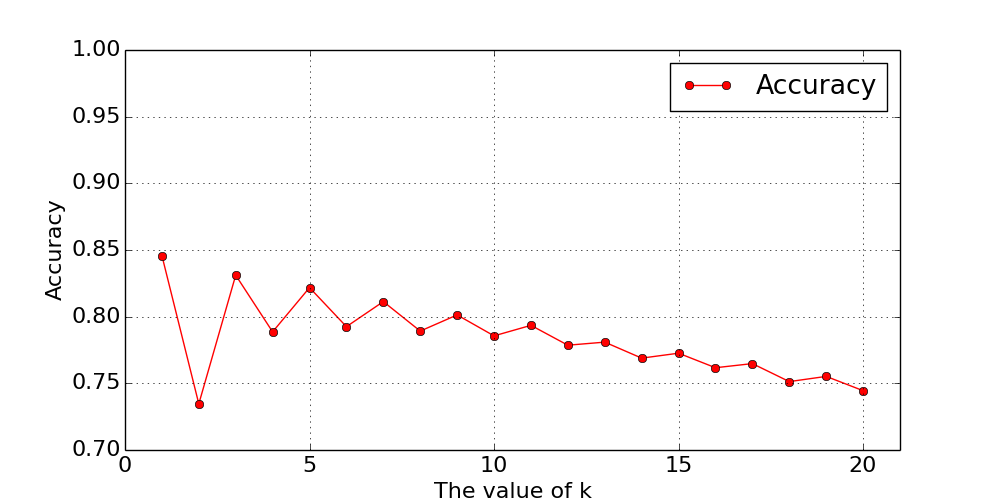
\includegraphics[]{figure_2.png}}
      \caption{Plot for $sin(w * \pi 2^{-k})$ where $w = 1$. }
      \label{fig:2}
     \end{center}
    \end{minipage}

    \begin{minipage}{0.01\hsize}
    \end{minipage}

%    \begin{minipage}{0.5\hsize}
%     \begin{center}
%      \scalebox{0.33}
%      {\includegraphics[]{figure_3.png}}
%      \caption{\label{fig:3}}
%     \end{center}
%    \end{minipage}

  \end{tabular}
 \end{center}
\end{figure}

According to \ref{fig:2}, we can see that as $w$ increases, the width of the wave become thinner. Since I am multiplying, and the wave length of $\sin(w2^{-k})$ gets thinner as $w$ gets bigger, we have to make sure that $w$ is monotonically increasing.

My strategy was to update the weights in different way according to the misclassification pattern. If the example is misclassified as ``-1'', then $w = w * \frac{5\pi}{2}$. Else, $w = w * \frac{3\pi}{2}$. The values are adjusted to classify the first training data in the first iteration, but in practice, even if the updating values are swapped, it still converges. 

%$$
%\mbox{one cycle of the wave }= \sin(4\pi)
%$$
%$$
%-1 \mbox{while } sign(\sin(4\pi)) \leq x \leq sign(\sin(4\pi + pi))
%$$
\end{document}

